\documentclass[11pt]{article}
\usepackage{amssymb}
\usepackage[english]{babel}
\usepackage{fullpage}
\usepackage{graphicx}
\usepackage{hyperref}

\def\titre{}
\def\auteur{}
\def\courriel{}
\makeatletter

\title{Polytechnique Montreal\\LOG8415 : Advanced Concepts of Cloud Computing\\Laboratory 2\\MapReduce with Hadoop on AWS}


\author{
    Christian Njon\\
    Dimitry Kamga\\
    Michelle Sepkap Sime\\
    Rui Jie Li
}

\date{4th November 2022}


\begin{document}
\maketitle

\maketitle

\section{Introduction}

\section{Hadoop and Spark}
MapReduce on Hadoop and Spark using AWS is the subject of the second assignment for the LOG8415E course. The objectives of this assignment are to acquire some skills with large data technologies and learn to integrate issues and methods into the MapReduce paradigm. Four primary sections make up this report. First, we will discuss our Word Count application in Hadoop trials. Second, we compare Hadoop's performance to that of Linux. Third, we compare the performance of Spark and Hadoop on AWS. We wrap up by outlining our algorithm and the MapReduce tasks we used to tackle the social network problem. We present our recommendations for connections based on the algorithm.

\subsection{Experiments with Word count Program}
Here, we first prepare the lab setting by setting up Hadoop on our computer. We adhered to the assignment's guidelines. Our major goal was to use Hadoop to process a pg4300.txt file. So that the Hadoop Name Node and Data Nodes could share the file, we downloaded it to a local directory and then moved it to the Hadoop Distributed File System (HDFS).
The data file pg4300.txt was then moved to the "input" directory we had just created in the Hadoop Distributed File System (HDFS).
The wordcount.java program from the Hadoop example directory was then executed. The screen capture of the Hadoop settings on localhost is shown in Figure~\ref{fig:hadoopgui1} and Figure~\ref{fig:hadoopgui2}. The input directory containing the pg4300.txt file is shown in Figure~\ref{fig:hadoopgui3}.

\begin{figure}
    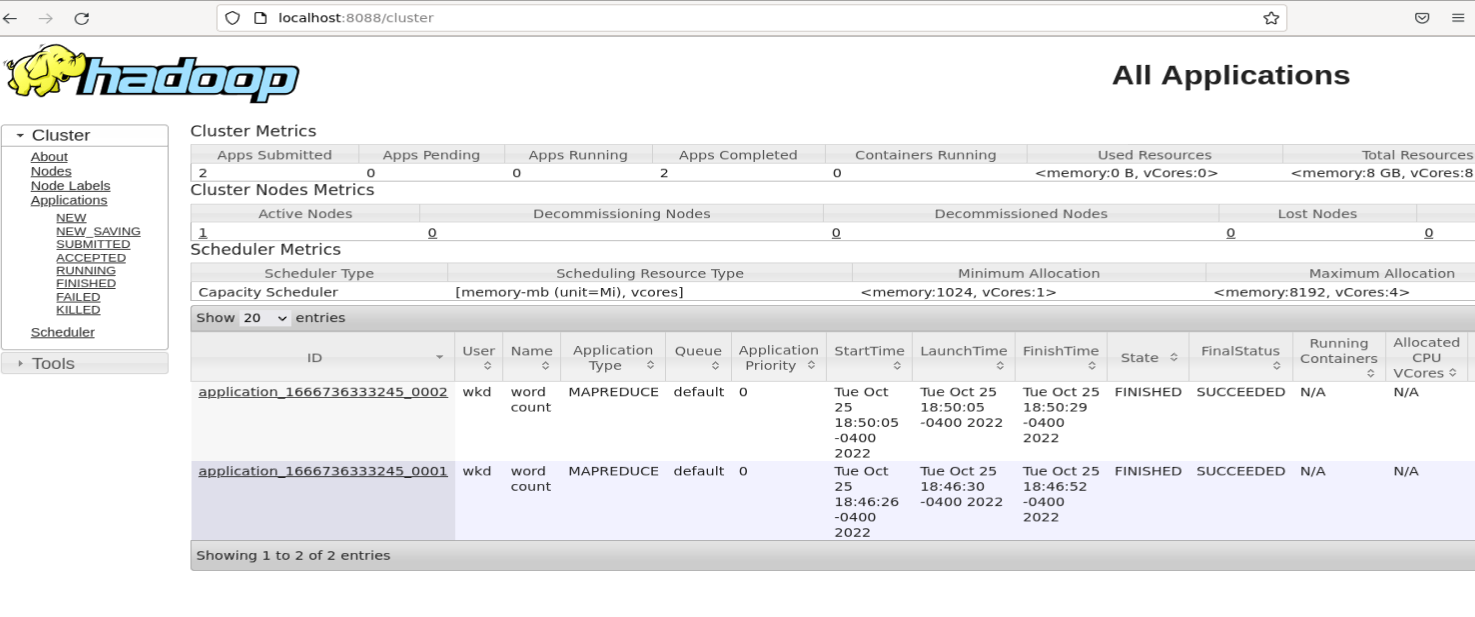
\includegraphics[width=\linewidth]{hadoop_gui1.png}
    \caption{Hadoop Overview GUI - part1}
    \label{fig:hadoopgui1}
\end{figure}

\begin{figure}
    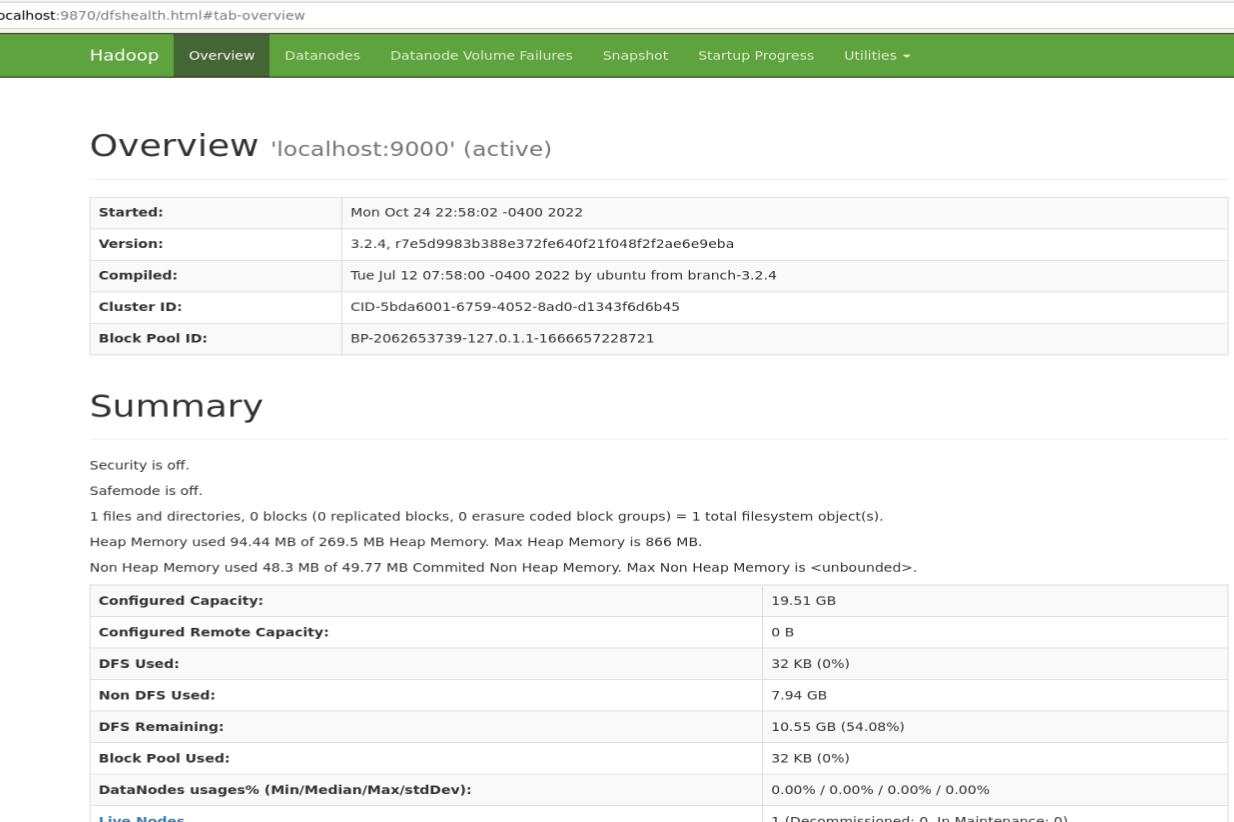
\includegraphics[width=\linewidth]{hadoop_gui2.png}
    \caption{Hadoop Overview GUI - part2}
    \label{fig:hadoopgui2}
\end{figure}

\begin{figure}
    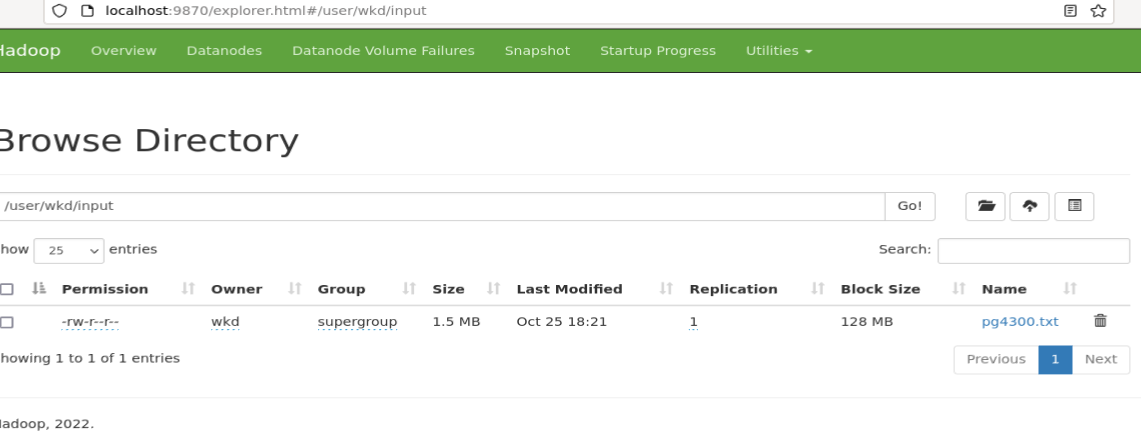
\includegraphics[width=\linewidth]{hadoop_gui3.png}
    \caption{Hadoop directory}
    \label{fig:hadoopgui3}
\end{figure}

\subsection{Performance comparison of Hadoop vs. Linux}
In this part, we compared the word frequency computation capabilities of Hadoop with those of a standard PC running Linux. \newline
First we installed Hadoop and spark binaries.
Then we ran the wordcount program with hadoop on a copy of James Joyce’s Ulysses book page 4300 available at [1]. The wordcount program just counts how many times each word appears in a file. We also di the same on an AWS M4.Large instance using the command cat ./pg4300.txt $\vert $tr ' ' '\textbackslash n' $\vert $sort $\vert $uniq -c. Here are the results:
\begin{table}[h!]
    \caption{Hadoop vs Linux Wordcount}
    \label{tab:table1}
    \begin{tabular}{|l|r|}
        \hline
        \textbf{Hadoop} & \textbf{Linux}\\
        5.961s & 0.170s\\
        \hline
    \end{tabular}
\end{table}

\vspace*{0.5cm}
\noindent
As we can see, Linux completes the task more quickly than Hadoop. This is expected because Hadoop is acceptable or suitable for more sophisticated tasks than the one we used.

\subsection{Performance comparison of Hadoop vs. Spark on AWS}
We first set up our infrastructure as follows in order to compare the performances of Hadoop and Spark on AWS. We generated a M4.large linux Ubuntu instance , and we installed Hadoop 3.3.4 and Spark on it. We confirm the installation of all necessary packages. Then, we timed the WordCount program's execution on both Hadoop and Spark machines three times across the entire dataset. We used 9 text files for this comparison, they can be found in the Datasets folders in Lab2, index shown in Figure~\ref{fig:dataset}.
\begin{figure}
    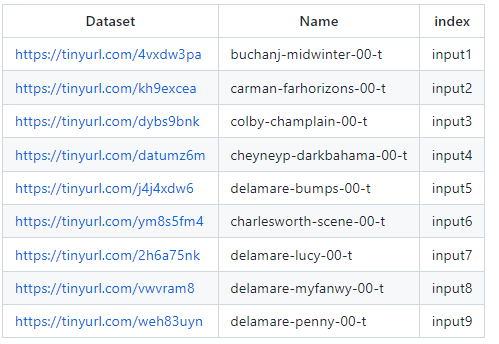
\includegraphics[width=\linewidth]{dataset.png}
    \caption{Dataset index}
    \label{fig:dataset}
\end{figure}

\vspace*{0.5cm}
\noindent
Spark was anticipated to be considerably faster than Hadoop since it makes use of random access memory and this is the case indeed.
The results are shown in the Figure~\ref{fig:plots}.
\begin{figure}
    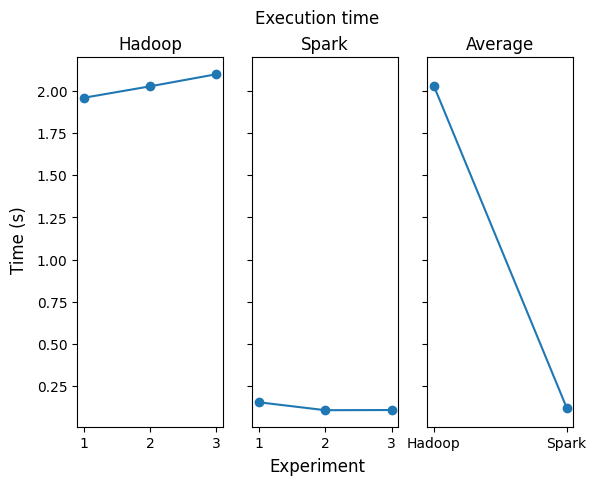
\includegraphics[width=\linewidth]{execution_time.png}
    \caption{Performance comparison of Hadoop and Spark}
    \label{fig:plots}
\end{figure}

\vspace*{0.5cm}
\noindent
This experiment and the last one has been automated through a bash script described in the section~\ref{instructions}.

\section{Instructions to run the code}  \label{instructions}

The entry point of the project is the bash script \textbf{run.sh} located at the root level of Lab2 folder. What this script does is simply to schedule all steps that need to be done in order to have the performance results.
First, it checks whether the necessary credentials (aws\_access\_key\_id, aws\_secret\_access\_key, aws\_session\_token) and the region config are set. The check proceeds this way :
\begin{itemize}
\item Check if the default values have been set by aws cli by means of configure command,
\item If not, check if they are available among the environment variables,
\item If they aren't, get them from user input and export them to make them available for upcoming scripts.
\end{itemize}
Once credentials and minimum config are set, we create and activate a python virtual environment to install dependencies so that user python environment remains unchanged. Then, we deploy and setup infrastructure, it is composed of one M4.Large instance and a security group to allow SSH access. If the setup fails to complete, we teardown already created infrastructure and exit. During the setup we store SSH private key and public IP address for later use.

\vspace*{0.5cm}
\noindent
Infrastructure step completed, we go to the next one which is executing hadoop and spark programs via SSH (using paramiko python library), saving execution time to files (results.txt for hadoop vs linux, hadoop.txt for hadoop performance and spark.txt for spark performance) that are also retrieved by SSH. We save those results in files and plot them. Finally, as soon as we have all we wanted, the infrastructure is destroyed and the virtual environment deactivated.


\section{References}
[1] Gutenberg textual data. http://www.gutenberg.org/cache/epub/4300/pg4300.txt.\newline
[2] Github repo. https://github.com/MichelleSS1/Lab8415

\end{document}
